\documentclass[12pt]{article}
\usepackage{graphicx}
\usepackage{setspace}
\usepackage[]{hyperref}
\usepackage[super]{nth}
\usepackage{pdflscape}
\usepackage{rotating}
\usepackage{listings}
\usepackage{enumitem}

%\usepackage{bera}% optional: just to have a nice mono-spaced font
\usepackage{listings}
\usepackage{xcolor}
\usepackage[title]{appendix}


\colorlet{punct}{red!60!black}
\definecolor{background}{HTML}{EEEEEE}
\definecolor{delim}{RGB}{20,105,176}
\colorlet{numb}{magenta!60!black}

\lstdefinelanguage{json}{
	basicstyle=\normalfont\ttfamily,
	numbers=left,
	numberstyle=\scriptsize,
	stepnumber=1,
	numbersep=8pt,
	showstringspaces=false,
	breaklines=true,
	frame=lines,
	backgroundcolor=\color{background},
	literate=
	*{0}{{{\color{numb}0}}}{1}
	{1}{{{\color{numb}1}}}{1}
	{2}{{{\color{numb}2}}}{1}
	{3}{{{\color{numb}3}}}{1}
	{4}{{{\color{numb}4}}}{1}
	{5}{{{\color{numb}5}}}{1}
	{6}{{{\color{numb}6}}}{1}
	{7}{{{\color{numb}7}}}{1}
	{8}{{{\color{numb}8}}}{1}
	{9}{{{\color{numb}9}}}{1}
	{:}{{{\color{punct}{:}}}}{1}
	{,}{{{\color{punct}{,}}}}{1}
	{\{}{{{\color{delim}{\{}}}}{1}
	{\}}{{{\color{delim}{\}}}}}{1}
	{[}{{{\color{delim}{[}}}}{1}
	{]}{{{\color{delim}{]}}}}{1},
}

\setlist[1]{itemsep=-5pt}
\usepackage[square,numbers]{natbib}

\hypersetup{backref,
			pdfpagemode=FullScreen,
			colorlinks=true,
			urlcolor=blue,
			citecolor=red}
\renewcommand{\baselinestretch}{1.2}

\begin{document}
\title{\Large A mediator system for robotic applications\\
[6mm]
\Large Rubanraj Ravichandran\\
[12mm]
\Large Master Thesis Proposal\\
\small Master of Autonomous Systems\\
[12mm]
\Large Department of Computer Science\\
University of Applied Sciences Bonn-Rhein-Sieg\\
[12mm]
\Large Supervisors:\\
Prof. Dr. Erwin Prassler\\
\Large Advisors:\\
Nico Huebel\\
Sebastian Blumenthal
}
\date{\today}
\maketitle
\newpage
\section{Introduction}

Robots generate large amount of data from different types of sensors attached to it and also from its hardware components. In our previous research work \cite{ravichandranworkbench}, we have conducted an extensive qualitative and quantitative analysis to find better databases and architectures that effectively store these data and consume it for further operations. Results from our previous work shows that, a single database is not suitable for every robotic scenarios. For example, in terms handling large BLOB data, mongoDB stored them faster but reading the data was slower compared to couchdb \cite{ravichandranworkbench}. Also, to complete a given task robots depends on multiple source of information from internal sensors, as well as external sources for example world model, kinematic model, etc.. 

Adoption of multiple databases for robotic applications requires unique way of mediation to view multiple databases as a single federated database. Mediator approach helps to integrate data from different sources and produce a single result back to robots. Mediator abstracts the information of how data is being stored in different data sources from robot, and allows robotic applications stream data to mediator independent of databases used in the back-end.

To Map the data generated by robots with multiple databases, mediator system requires a proper data model predefined in the context of robotic applications. Modeling robot generated data helps to generalize the structure of data and defining relations between different objects in the robot systems. If we have a well defined robotic data models, then mediator will get the ability to mutate or query data from different data sources. Also it is important that, these data models should be extended to any robotic use-cases.

As mentioned in these papers \cite{ahmed1991pegasus,fahl1993amos,arens1996query,chawathe1994tsimmis,chawathe1994tsimmis,shoens1993rufus}, mediators are being used to integrate data from different data sources and few architectures supports single data model (e.g SQL), and others supports for different data models (e.g SQL,NoSQL, document store, etc..). Also, they are differ from query languages, ease of implementation, components used in their architecture. This project mainly focus on defining semantic based models for sensor data to make it more inter-operable with other systems or even in multi robot systems, and implementing a mediator system which act as a middle-ware between robots and databases. 

\section{State of the art analysis}

\subsection{Semantic Data model}
\citet{su2014connecting} highlights the interoperability issues in IoT sensor data and also says that these data should be useful for multiple applications rather than dependent on specific domain. To make the machines interpret the meaning of sensor data, author suggested to use Semantic Web technologies such as Resource Description Framework (RDF). Even though SenML is an evolving technique to model to sensor data, but it is lacking reasoning capabilities and interoperability with other devices. To overcome the issues in SenML generic model, author proposes a technique to represent IoT sensors as a Knowledge Based Systems by transforming SenML to Resource Description Framework. 

As an advantage, the transformed data can be analyzed and helpful to take more meaningful actions. 

SenML is specially designed for resource constrained devices, hence additional information to contextually understand the data has be not excluded intentionally. Each entry of SenML data should have the sensor parameter name and other attributes such as time, value, etc. Also it supports custom attribute called Resource Type (rt) to let the users add their own attributes and this allow users to include contextual information.

\subsection{Mediator architectures}
\citet{fahl1993amos} proposed an active mediator architecture to gather in
formation from different knowledge base and combine them to a single response. AMOS\footnote{\label{amos}Active Mediators Object System} architecture uses Object-Oriented approach to define declarative queries. This distributed architecture involves multiple mediator modules to work collaboratively to collect the required piece of information and produce final result. Primary components of AMOS architecture are,
\begin{itemize}
	\item Integrator - Gather data from multiple data sources that have different data representations.
	\item Monitor - Monitor service always watch for any data changes and notifies the mediators. This is helpful in the case where system needs an active updates to change its current task.
	\item Domain models represents the models related to application which helps to access data easier from any database through a query language.
	\item Locators helps to locate mediators in the network.
\end{itemize}


Integrator module is built with two internal components called IAMOS\footnote{\label{amos}Integration Active Mediators Object System} and TAMOS\footnote{\label{amos}Translation Active Mediators Object System}. 
First Integration AMOS parse the query and send individual requests to Translational AMOS modules which are responsible for heterogeneous data source.
Then,all TAMOS modules return the individual results to IAMOS for integrating all the results. To query multi databases from IAMOS, IAMOS servers are mapped with TAMOS servers with the help of Object-Oriented query language.


\citet{ahmed1991pegasus} developed a heterogeneous multi-database system called Pegasus that supports multiple heterogeneous database systems with various data bases models, query languages and services. Pegasus predefines its domain data models based on object oriented approach and also supports programming capabilities. These objects are created and mapped with the types and functions with the help of HOSQL\footnote{\label{myfootnote}Heterogeneous Object Structured Query Language} statements. HOSQL is a declarative object oriented query language which is used by Pegasus to manipulate data from multiple data sources.



Pegasus system supports two types of data sources, local and native data sources. Whenever a new data source joins Pegasus system, schema integrator module imports schema from data source and update its root schema with the new schema types. The final integrated schema shows the complete blueprint of the different data sources participates in the data integration. Pegasus system work-flow is comparatively similar to AMOS architecture, but they use different query language and data modeling strategies.

\citet{chawathe1994tsimmis} developed project Tsimmiss extract information from any kind of data source and translates them to a meaningful common object. Unlike AMOS and Pegasus, Tsimmiss follows a straight forward approach to define the data model which is a self-describing object model. Each object must contain a label, type and value itself. Label can be used by the system to understand the meaning of the value and type shows the observed value type. Objects can be nested together to form a set of objects. 

Tsimmiss tool offers a unique query language called OEM-QL and this language follows the SQL query language pattern to fetch the data from mediators. Mediators resolves the query and send separate requests to respective data sources to retrieve the information and merge them together to give a single response back to user. During data integration process, Tsimmiss removes possible duplicates to avoid redundancy in the response. Also, Tsimmiss bundles a default browser tool to query data using OEM-QL language.

In the articles discussed above, mediators are targeted to extract information from different data sources that could be different databases or data from file-system. But Rufus system proposed by \citet{shoens1993rufus} focus only on semi structured data stored in file system for example documents, objects, programming files, mail, binary files, images etc. Rufus system classifier automatically classifies the type of file and apply a scanning mechanism on those files to extract the required information and transform them to the appropriate data model which is understandable by Rufus system. Rufus can classify 34 different classes of files. In terms of query language, Rufus can apply simple object predicates and finding text from the extracted information from the documents or files.

\citet{papakonstantinou1996medmaker} proposes a Mediator Specification Language that helps the mediator to understand the schema and integrates the data from unstructured or semistructured source. MSL overcomes the major problems in existing mediator systems for example,
\begin{itemize}
	\item Schema domain mismatch 
	\item Schematic discrepancy
	\item Schematic evaluation
	\item Structure irregularities
\end{itemize}

During translation of original information from different sources to a single object it should be important that, all data sources should have the required attribute and the name of the attribute should be same. Otherwise, mediator system will not be able to process the information to a single answer.  External predicates and Creation of the Virtual Objects in MSL solves the problems mentioned above.

\citet{arens1996query} built a mediator which is flexible to map domain level query different data-sources and efficient to plan the query execution to reduce the overall execution time. Information source models provides relations between the super class and subclasses, and also the mapping between the domain models and information from heterogeneous sources. SIMS uses Loom as a representational language to make objects and relationship between them. SIMS supports parallel query access plan that makes the mediator to access information independent of data sources and the user will get the final answer as quick as possible.

Many mediator systems developed in the past to support integrating heterogeneous information from different data sources. All of them built with different architectures, query language, and execution optimization. In our mediator approach we focus mainly on,
\begin{itemize}
	\item How different type of robot generated data will be stored in multiple data sources?
	\item A unique context based data model to represent the components attached with each robot and data generated by them.
	\item Semantic query language to communicate with mediator. Unlike traditional query languages we would like to attempt new way of querying data, for example Graphql.
	\item GUI tool to visualize and analyze the robot generated data in a meaningful way.
\end{itemize} 

 

\section{Problem Formulation}

Our previous work results reveals not all databases reacts in a similar fashion for different heterogeneous data from robotic applications. Also, there are no concrete data models has been defined in the context of robotic applications. For example, black box designed for ROPOD project uses mongoDB to store data from different sources such as Ethercat, Zyre, ZMQ, and ROS topic. The data is being transformed in to a simple flatten json document to store the values. These documents are stored under a single collection which is created for each ROS topic or other sources. Each document holds only the information of value generated by the sensors or application itself, but these values are not useful without additional details for example, who created the data, if it is a robot then what type of robot generated this data from which location?, then in what context other system should interpret this data.

For example in the black box, geometry\_msgs/Pose ROS topic will be flattened to a simple json document which have the following format.

\begin{lstlisting}
	double timestamp
	double position/x
	double position/y
	double position/z
	double orientation/x
	double orientation/y
	double orientation/z
	double orientation/w
\end{lstlisting}

In the above format, 'position/x' is a key and the value will be attached with it. Now only with position x,y,z and orientation x,y,z,w, other system which consumes this data would not be able to say who generated this data or at which location this data is being generated and if the other system is doing mathematical calculation, then this data is missing it own context such as unit, dimensions, etc.


%(contact alex or santhosh to see the current implementation and complete the problem here)

In terms of supporting multiple databases setup for robots,  there is no systematic approach to store and retrieve data from external sources and, a well defined data model that can map components and sensors to a robot and also with the world model.
In this case, there is no mediator has been developed before to connect between robots and databases with different data model.

%These are the major problems will be discussed and addressed in this work,
%\begin{itemize}
%	\item Data model for robotic applications
%	\item Implementation of single mediation layer to connect between robots and databases (different data model)
%	\item Unique query language that can be used by robots to talk with different databases via mediator.
%\end{itemize}

\section{Approach}

To find the best data models for robotic applications and build a scalable mediator, we begin with SOA analysis to find out approaches that has been followed through before for similar data integration applications. After defining the data model, list of recent querying techniques will be collected and reviewed based on the features and possibility of adopting them with the mediator as a base. For review we would like to consider current well known querying techniques such as Graphql, and Falcor. At first, our mediator will support only the databases which are selected based on the results from our previous research work \cite{ravichandranworkbench} and other data-sources used by ROPOD such as OpenStreetMap. Then, schema's will be defined to map the data being generated by the robot and the data sources. To reduce the complexity of identifying appropriate data-sources by the robot, in our architecture mediator will dynamically choose the data-source respective to the type of data that robots want to store and retrieve. Still the configuration will be adjustable according to the scenarios. Finally to visualize the integrated data from mediator in a meaningful way, a GUI application will be developed based on Node.js stack.

\section{Workplan}
This work-plan shows the major decomposition of the work-packages, start time and end time. This project starts on October \nth{15}, 2018 for 6 months duration and ends on April \nth{16},2018.
\newpage
\subsection{Work packages}
\begin{figure}[h!]
  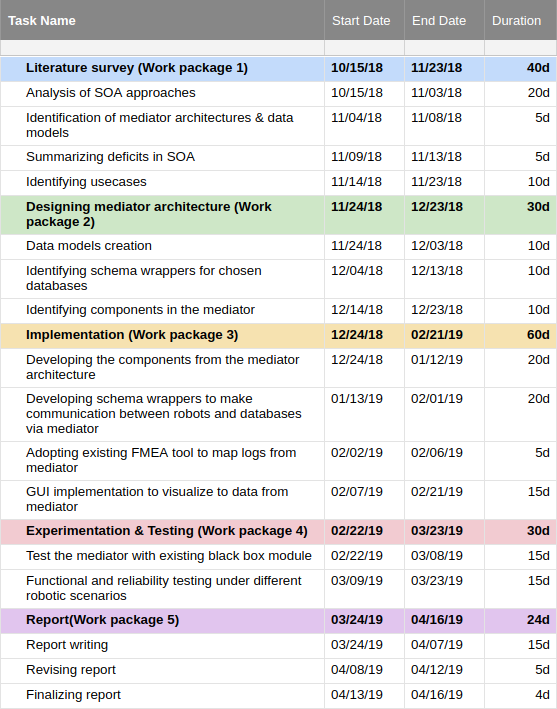
\includegraphics[width=\linewidth,height=17cm]{wp_v1.png}
  \caption{Work packages}
  \label{fig:work_packages}
\end{figure}


\begin{landscape}
	\subsection{Gantt Chart}
	\begin{figure}[h!]
	  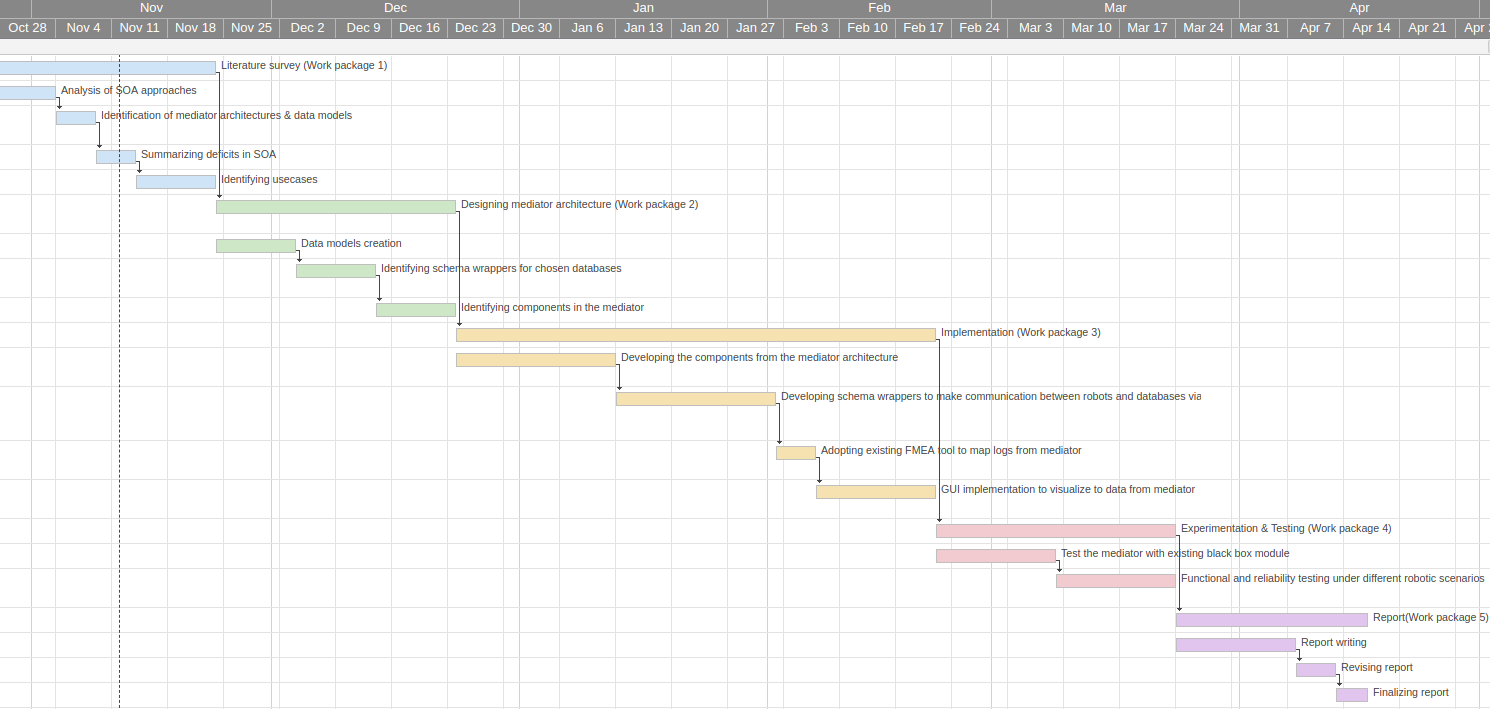
\includegraphics[width=20cm,height=11cm]{time_line_v1.png}
	  \caption{Gantt Chart}
	  \label{fig:gantt_chart}
	\end{figure}
\end{landscape}

\newpage
\section{Deliverables}
\subsection{Minimum}
\begin{itemize}
\item Report on state of the art analysis.
\item Collection of existing mediator architectures which can be adopted to robotic applications.
\item Data modeling in the context of robotic applications.
\item Finding unique and semantic query language to communicate with mediator.
\end{itemize}
\subsection{Expected}
\begin{itemize}
\item Designing and implementing mediator system that supports storing and retrieving robot generated sensor data from different data sources dynamically.
\item Suitable data model and relationships for multi robot use-cases.
\end{itemize}
\subsection{Maximum}
\begin{itemize}
\item Developing a GUI tool to interactively communicate with mediator and visualize the sensor data in a meaning way.
\end{itemize}

\newpage
%\section{References}
\bibliography{bibfile}
\bibliographystyle{agsm}

\newpage


\end{document}
